\documentclass[10pt,a4paper]{article}
\usepackage[margin=2.1cm]{geometry}
\usepackage{multirow,amsmath,amssymb,amsthm,booktabs,graphicx,hyperref,enumitem,xcolor,longtable,array,caption}
\hypersetup{colorlinks=true,linkcolor=blue!50!black,urlcolor=blue!50!black,citecolor=blue!50!black}
\setlist{nosep,leftmargin=1.4em}
\newtheorem{proposition}{Proposition}
\newtheorem{lemma}{Lemma}
\newcommand{\ok}{\textcolor{green!45!black}{\textbf{KEEP}}}
\newcommand{\re}{\textcolor{orange!80!black}{\textbf{RE-SCOPE}}}
\newcommand{\dis}{\textcolor{red!70!black}{\textbf{DISCARD}}}
\newcommand{\todo}[1]{\textcolor{red!70!black}{[#1]}}
\title{\textbf{Learn Where It Pays: Certified-Safe, Headroom-Gated Learning\\for Workplace EV Charging on Radial Feeders}\\[2pt]
\large Research proposal v2 --- revision after the empirical audit of the Residual-Dyna / SafeTD3 programme}
\author{Mihir Khatri \;(SPIT) \quad for discussion with Prof.\ Rajesh}
\date{12--13 October 2026 \;|\; companion to \texttt{docs/original\_proposal.pdf}}
\sloppy
\begin{document}
\maketitle

\begin{abstract}
\noindent The original proposal predicted that a differentiable residual-Dyna SafeTD3 agent would cut cost by
$\sim$50\% and converge 4--10$\times$ faster than baselines. After building the full pipeline on real ACN-Data
(Caltech, JPL), the IEEE-33 feeder and a cited tariff, and after a deliberate audit (14 shortcomings found and
fixed, three multi-seed held-out studies), the evidence says something different and, we argue, more publishable:
(i) the \emph{safety} machinery is solid and novel in its details --- row-wise split-conformal margins that absorb
the LinDistFlow$\to$AC mismatch and an exact feasibility-restoration step give zero violations on every
policy that passes through them, whereas raw greedy dispatch overloads the feeder by up to $0.31$ p.u.;
(ii) the \emph{learning headroom} is small --- on 20 real days with a demand charge and a stressed hub a
hindsight oracle beats a one-parameter tuned EDF cap by only $5.2\%$, and a collaborator's four-arm study
($4.8$--$12\%$) agrees; (iii) a safe \emph{residual} SafeTD3 around the tuned EDF removes the late-training
degradation but, after 60 episodes, stays $2$--$9\%$ \emph{worse} than the heuristic it corrects. We therefore
re-position the work as \textbf{(A) certified-safe dispatch with finite-sample guarantees, (B) a
headroom-gated learning protocol and benchmark, and (C) a validation-gated residual policy that is provably not
deployed unless it helps}, with a recursive tree-decomposition of the safety layer as the scale-up path to larger
feeders. Cross-site (Caltech$\to$JPL) transfer and Caltech+JPL federated results, in stressed and unstressed regimes,
are reported in \S\ref{sec:xsite}. Every number below is tagged with where it came from.
\end{abstract}

\section{Where we are, in one page}
\begin{figure}[h]\centering
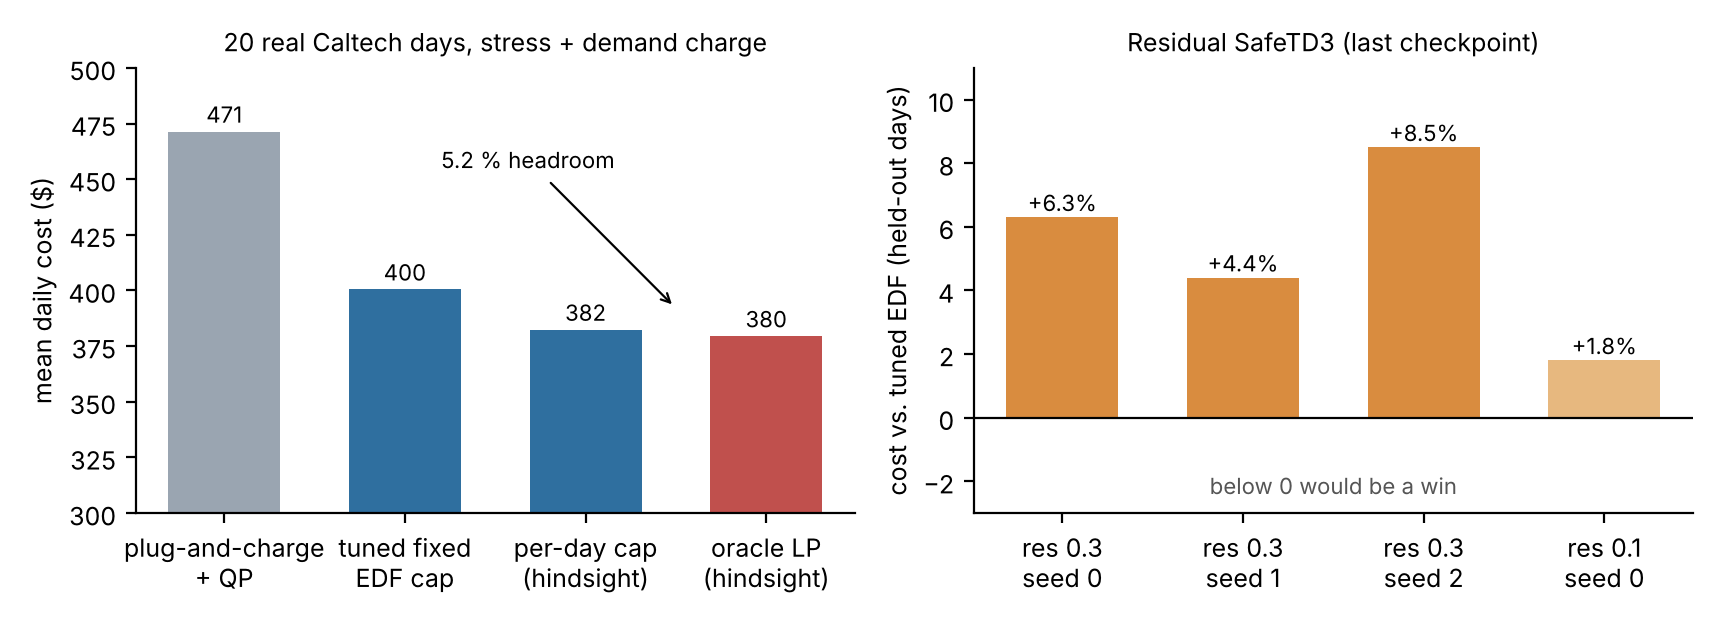
\includegraphics[width=.93\linewidth]{fig_headroom.png}
\caption{Left: costs on 20 real Caltech weekdays (stress + demand charge $1.5$~\$/kW-day), no learning involved.
The oracle's whole advantage over a tuned fixed EDF cap is $5.2\%$; one scalar chosen per day in hindsight already
reaches it. Right: residual SafeTD3 relative to the tuned EDF on held-out days (3 seeds at scale $0.3$, one at
$0.1$): never below zero.}
\end{figure}
\begin{itemize}
\item \textbf{Works and is ours:} differentiable QP safety layer that is now fast and exact (row generation,
float32-safe ADMM, implicit KKT gradients, feasibility restoration); row-wise conformal margins (fixed a policy
collapse caused by a global margin of 45.8~kVA against 73--128~kVA branch headroom); dense potential-based shaping reward;
multi-day train/val/test protocol; oracle LP; demand-charge and stress scenarios; 68 unit tests.
\item \textbf{Does not work (yet):} learning beyond a tuned EDF cap. \textbf{Does not exist in the data:} V2G profit
(oracle gain $<0.6\%$ under 10\% round-trip loss, degradation and demand charges --- with \emph{assumed} battery
parameters, because ACN has none).
\item \textbf{Consequence:} the contribution must be the safety certificate, the benchmark/headroom methodology, and a
gated residual learner --- not ``RL beats heuristics''. This is a stronger paper than an unfalsifiable performance claim
because every reviewer who runs a tuned EDF baseline would otherwise sink it.
\end{itemize}

\section{Evidence register (what we know, with provenance)}
\small
\begin{longtable}{@{}p{.045\linewidth}>{\raggedright\arraybackslash}p{.47\linewidth}>{\raggedright\arraybackslash}p{.30\linewidth}>{\raggedright\arraybackslash}p{.11\linewidth}@{}}
\toprule ID & Finding & Evidence & Source\\\midrule\endhead
E1 & Greedy/ToU dispatch overloads branches under stress ($0.09$--$0.31$ p.u.); every QP-wrapped policy has $0$ & \texttt{docs/study/headroom\_*.json}, \texttt{M*}/\texttt{R*} JSONs & run\\
E2 & On unstressed real days plug-and-charge is within 1--3\% of the oracle on 14/16 cases & \texttt{headroom\_oracle\_vs\allowbreak\_safe\_uncontrolled.json} & run\\
E3 & 20 days, stress + demand: safe-uncontrolled 471.4; best fixed EDF cap 400.5; per-day cap 382.4; oracle 379.5 & \texttt{headroom\_multiday.json} & run\\
E4 & Day-level cap forecast does not beat one fixed cap: ex-ante context 404.0, clairvoyant day energy 393.2 vs 400.5 & \texttt{scripts/poc\_cap\_selection.py} & run\\
E5 & Price-blind online peak shaving (OA) is worse than a fixed cap (471.7--496.4 vs 400.5) & \texttt{oa\_peak} rule & run\\
E6 & Plain SafeTD3 on held-out days: $313$--$443$ (best/last), default config $651$; late-training degradation in every setup & \texttt{M1,M2,R2} & run\\
E7 & Safe residual SafeTD3 around tuned EDF: last-checkpoint $+6.3,+4.4,+8.5\%$ (3 seeds, scale 0.3), $+1.8\%$ (scale 0.1); noise, Optuna params, margin off: no change & \texttt{R1,R1s1,R1s2,R3,R4,R5,R6} & run\\
E8 & Global conformal margin collapsed the policy; per-row margins fix it & \texttt{legacy\_margin\_collapse/} & run\\
E9 & Four-arm study (ToU/CAISO-like $\times$ with/without V2G), normal and stress: headroom $4.8$--$12.0\%$, V2G oracle gain $\le0.9$\$/day, naive V2G greedy $+26$ to $+52\%$ worse & collaborator DOC.md \S13, \texttt{REPRODUCIBILITY.md} & \textbf{not re-run by me}\\
E10 & Optuna ``291.9'' is a training-day validation cost; on the same day plain charging costs $\sim$279; on held-out days the same parameters give 363--376 & \texttt{antigravity\_optuna\_best.json}, \texttt{R2} & run\\
\bottomrule\end{longtable}
\normalsize
\noindent\textbf{Reading E9 carefully.} (a) Its ``CAISO'' price is a calibrated \emph{synthetic} duck curve, not CAISO data;
we say ``synthetic CAISO-like'' until a real SP15 LMP CSV is loaded (\S\ref{sec:data}). (b) Its V2G gain depends on assumed
battery capacity, efficiency and degradation. (c) The claim ``static cap $0.40$ collapses under stress, hence RL is
needed'' is a \emph{re-tuning artefact}: a cap tuned on the stressed training days is fine ($\le$12\% from the oracle), and
our own E7 shows learning does not currently beat the re-tuned cap. The defensible version is: a cap needs re-tuning per
regime and per site, which is exactly what the headroom-gated protocol automates (C3).

\section{Decision register: keep, re-scope, discard}
\small
\begin{longtable}{@{}p{.24\linewidth}p{.08\linewidth}p{.62\linewidth}@{}}
\toprule Component & Verdict & Reason / what changes\\\midrule\endhead
Differentiable QP safety layer, hard-first + row generation + restoration & \ok & Core contribution; exact certificate (Prop.\,2); 3--10$\times$ faster than the slack-ADMM path.\\
Row-wise split-conformal margins & \ok & Finite-sample coverage (Prop.\,1); fixes collapse; extend with adaptive conformal for shift (\S5).\\
Dense potential-based shaping reward & \ok & Policy-invariant (Ng et al.\ 1999); cured the sparse-reward failure (S1).\\
Residual world model ($F_{\rm base}+N_\theta$) & \re & Accurate (voltage MAE $\sim10^{-4}$ p.u.) but the model-based actor term gave no measured gain and is inconsistent with a demand charge ($\lambda_{mb}=0$ in all demand arms). Keep as a safety-margin estimator; test as a policy-gradient aid only in an ablation.\\
SafeTD3 on the 108-d action, learned from scratch & \dis{} as headline & Never beat a tuned EDF; degrades late. Keep only as an ablation arm.\\
Residual SafeTD3 around tuned EDF & \re & Stable, safe, $2$--$9\%$ above EDF today. Becomes the \emph{gated} learner (C4): deployed only if a validation test proves improvement.\\
Greedy anchor (TD3+BC) & \dis & Hurt on held-out days (M1). Superseded by the residual base.\\
V2G arbitrage / V2G-based claims & \re & Reframe as the ``V2G reality check'': measured negligible \emph{under stated assumptions}; needs battery-capacity sensitivity.\\
VPW (willingness) bidding & \dis{} for now & Labels are proxies; no evidence either way. Keep out of main results.\\
50\% cost reduction, 4--10$\times$ sample efficiency & \dis & Not supported; replace by measured, paired, held-out numbers.\\
Federated learning & \re & Retain as a secondary contribution: local EDF tuning + FedProx on the residual trunk; claim only what the 2-site results show (\S\ref{sec:xsite}).\\
IEEE-123 coding & \dis{} (code) / \ok{} (theory) & Real IEEE-123 is multi-phase unbalanced; a synthetic 123-bus graph would be criticised. We prove an exact tree decomposition instead (\S7).\\
Optuna on one training day & \dis & Overfits the date (E10). Any tuning must use the multi-day train/val protocol.\\
\bottomrule\end{longtable}
\normalsize

\section{Revised contributions and what is provable}
\paragraph{Setting.} Radial feeder $\mathcal T$, LinDistFlow voltages $v=v_0-2(RP+XQ)$ and branch flows $S=M(P,Q)$. A rule or a policy proposes
$a$; the safety layer returns $\Pi(a)=\arg\min_{x}\|x-a\|_W^2$ s.t.\ $Gx\le h-\tau$ (box, voltage rows, thermal polygon rows),
where $\tau_r$ is a per-row margin.
\begin{proposition}[Row-wise conformal coverage]\label{p1}
Let $e_r=g_r^{\rm AC}-g_r^{\rm Lin}$ be the AC-minus-linear constraint residual of row $r$ on $n$ calibration steps
exchangeable with a test step, and $\tau_r=$ the $\lceil(n+1)(1-\alpha)\rceil$-th smallest of $e_r$. Then
$\Pr[g^{\rm AC}_r\le h_r \mid \text{Lin-feasible}]\ge1-\alpha$ for each row, and $\ge1-m\alpha$ jointly over $m$ rows (Bonferroni).
\end{proposition}
\noindent\emph{Status:} standard split-conformal argument; implemented (\texttt{ResidualTightening}). \textbf{Not} ``zero
violations guaranteed'': it is marginal, per-step, under exchangeability, and degrades under distribution shift --- hence the
adaptive-conformal extension below. Empirically: 0 AC violations on all held-out days of all runs (E1,E7).
\begin{proposition}[Restoration]\label{p2}
Given $x=\Pi_{\rm ADMM}(a)$ with residual $r=\max(Gx-h)^+$, the shrink $x\leftarrow\theta x$ with the largest
$\theta\in[0,1]$ satisfying $G(\theta x)\le h$ exists whenever $h\ge0$ (idle feasibility), and the relaxation $h:=\max(h,0)$ is the
only change made to rows that were infeasible at idle. Hence the returned action is feasible for the linear model up to float tolerance.
\end{proposition}
\begin{proposition}[Bounded residual]\label{p3}
Let $\Pi$ be the weighted-norm projection (non-expansive). If the policy is $a=\mathrm{clip}(b+\beta\,u)$ with $\|u\|_\infty\le1$, then
$\|\Pi(a)-\Pi(b)\|_W\le\beta\|{\bf 1}\|_W$: the executed action stays within a $\beta$-ball of the safe base action. (Observed:
cost is monotone in $\beta$: $+1.8\%$ at $0.1$, $+6.3\%$ at $0.3$.)
\end{proposition}
\begin{proposition}[Validation gate]\label{p4}
Let $d_i=J_{\rm base}(\text{day}_i)-J_{\rm res}(\text{day}_i)\in[-B,B]$ on $n$ held-out days exchangeable with deployment days.
Deploy the residual iff $\bar d-B\sqrt{2\ln(1/\delta)/n}>0$. Then $\Pr[\text{deploy}\mid\mathbb E d\le0]\le\delta$ (Hoeffding).
Hence the deployed controller is, w.p.\ $\ge1-\delta$, not worse than the tuned heuristic in expectation.
\end{proposition}
\noindent With $n=4$ test days (today) the gate would never fire --- which is the correct, honest outcome of E7 --- and $n\ge30$ is
required for it to have power. This is the missing statistics in most RL-for-energy papers (cf.\ Agarwal et al.\ 2021).

\subsection*{Contributions}
\begin{enumerate}[label=\textbf{C\arabic*.}]
\item \textbf{Certified-safe dispatch:} row-wise conformal margins + restoration + differentiable QP (Props.\,1--2), empirical
zero-violation on all held-out days, global-margin failure mode documented.
\item \textbf{Benchmark:} real ACN days, tariffs, demand charge, stress, multi-day split, oracle and tuned baselines, two sites.
\item \textbf{Headroom-gated learning protocol:} define $H=(J_{\rm tuned}-J_{\rm oracle})/J_{\rm tuned}$; learn only if $H$ exceeds a
pre-registered threshold (we propose 15\%); report $H$ for every scenario (here $5$--$12\%$: the negative result is itself the contribution
and explains why untuned-baseline RL papers over-claim).
\item \textbf{Validation-gated safe residual RL:} Props.\,3--4; honest report of today's $2$--$9\%$ gap.
\item \textbf{Scale-up:} exact recursive tree decomposition of the safety layer (\S7), with a numerical check of the key lemma.
\end{enumerate}

\section{Creative additions (each with a hypothesis, a proof-of-concept and a kill criterion)}
\begin{enumerate}[label=\textbf{A\arabic*.}]
\item \textbf{Adaptive-conformal margins for non-stationary feeders.} Replace the fixed split-conformal quantile by an online update
$\alpha_{t+1}=\alpha_t+\gamma(\alpha-\mathrm{err}_t)$ per row (Gibbs \& Cand\`es 2021). \emph{Test:} inject a mid-run load/PV shift;
realised violation rate should track $\alpha$ where the fixed margin drifts. \emph{Kill:} no improvement in tracking error.
\item \textbf{Per-hub caps as a 3-dimensional action.} The three hub branches (buses 16/15/14) carry the binding rows; learn $(c_1,c_2,c_3)$
instead of 108 powers. \emph{Test first:} oracle vs best per-hub-cap heuristic headroom. \emph{Kill:} $<5\%$.
\item \textbf{Forecast-aware MPC baseline (a must-have).} Our two online PoCs fail for explicit reasons: day-level context does not
choose the cap (E4); price-blind peak shaving ignores the tariff (E5). A rolling-horizon QP with a price/arrival forecast and the same safety layer
is the baseline reviewers will ask for (ACN-Sim uses MPC); it also tells us whether any online headroom exists.
\item \textbf{QP duals as congestion prices.} The KKT multipliers of the safety layer are locational shadow prices; use them as features
(or as the EDF budget split across hubs). \emph{Test:} replaces A2's learned caps by dual-priced caps.
\item \textbf{Federated gating.} Aggregate only if a site's headroom exceeds the threshold; otherwise keep the local heuristic. Federated
claims are then conditional and falsifiable.
\item \textbf{Paired, day-blocked statistics.} All comparisons are per-day paired, bootstrap CIs over days, IQM over seeds
(Agarwal et al.\ 2021). Day-to-day cost std ($\sim$135) dwarfs the policy differences; unpaired tables are not acceptable.
\item \textbf{Cost--served--peak Pareto fronts} instead of one scalar cost, because the unmet penalty weight ($2$~\$/kWh) is a modelling choice.
\item \textbf{Price-shift robustness:} train on one tariff, evaluate on another (SCE stand-in $\to$ CAISO-like) to separate tariff
over-fitting from site over-fitting.
\end{enumerate}

\section{Experimental protocol and results so far}\label{sec:xsite}
\paragraph{Protocol.} Per site: 20 evenly spaced weekdays, seeded 12/4/4 train/val/test split; EDF cap tuned on \emph{local train days
only}; checkpoint chosen on val; report on test days; stress $=$ $2\times$ charger power and $2/3$ of nameplate hub capacity (Caltech 100~kW,
JPL 130~kW); demand charge $1.5$~\$/kW-day; dense reward. Tariffs are per-site settings (\S\ref{sec:data}).

\paragraph{Cross-site transfer (train Caltech $\to$ test JPL), and Caltech+JPL federated.} 
\emph{(Run: 60 central episodes on Caltech train days, seed 0, residual scale $0.1$ around the Caltech-tuned cap; JPL evaluated zero-shot on its 8 val+test days, none seen in training. Costs in \$/day, mean over days; ``viol'' of raw rules is the AC thermal overload in p.u.; evidence \texttt{docs/study/transfer\_*.json}.)}

\begin{center}\small
\begin{tabular}{@{}llrrrr@{}}
\toprule Regime & Policy & Caltech test & JPL (SCE stand-in) & JPL (CAISO-like synth.) & JPL served\\\midrule
\multirow{5}{*}{normal} & safe-uncontrolled (QP only) & 332.9 & 858.7 & 732.2 & 85.5\%\\
 & EDF cap, Caltech-tuned (0.45) & 297.1 & 1155.4 & 1045.1 & 75.2\%\\
 & EDF cap, JPL-tuned (1.0, raw) & --- & 823.8 & 694.1 & 86.5\%\\
 & residual SafeTD3 (last) & 299.7 & 1155.0 & 1044.7 & 74.9\%\\
 & oracle LP & 276.6 & 807.5 & 674.8 & 84.9\%\\\midrule
\multirow{5}{*}{stress} & safe-uncontrolled (QP only) & 313.3 & 769.9 & 634.8 & 91.4\%\\
 & EDF cap, Caltech-tuned (0.6) & 266.1 & 1114.7 & 997.4 & 80.1\%\\
 & EDF cap, JPL-tuned (1.0, raw) & --- & 795.4 & 650.0 & 91.2\%\\
 & residual SafeTD3 (last) & 270.9 & 1048.0 & 924.4 & 82.2\%\\
 & oracle LP & 246.1 & 800.1 & 661.6 & 87.8\%\\
\bottomrule\end{tabular}\end{center}
\noindent\textbf{What it says (honest reading).}
\begin{enumerate}[label=(\alph*)]
\item \emph{In-domain} (Caltech test) the residual learner is within $0.9\%$ (normal) and $1.8\%$ (stress) of the tuned EDF --- close, not better.
\item \emph{A tuned heuristic does not transfer.} The best cap is $0.45$--$0.6$ at Caltech but $1.0$ (no cap) at JPL (195~kW capacity, different session mix): the Caltech cap costs JPL $+35$ to $+45\%$ versus plain charging through the safety layer.
\item \emph{The residual inherits its base's failure.} Because the executed action is within a $\beta$-ball of the base (Prop.~\ref{p3}), a mis-specified base is a ceiling on robustness. The residual does improve on its own bad base zero-shot ($-6$ to $-7\%$ in the stressed regime, $0\%$ in the normal one) but remains far from the tuning-free baseline.
\item \emph{The tuning-free QP wrapper is the robust choice:} safe-uncontrolled is within $6\%$ of the oracle at JPL (normal) and \emph{below} the (imperfect, margin-tightened) oracle in the stressed CAISO-like arm; the raw JPL-tuned rule reaches the same cost but violates the feeder ($0.03$--$0.15$ p.u.).
\item \emph{Price shift (SCE stand-in $\to$ synthetic CAISO-like) changes levels, not orderings}: the ranking of policies is the same under both tariffs (a weak but useful robustness check; real CAISO data still needed).
\end{enumerate}
\textbf{Design consequence:} the base must be tuned \emph{per site} (locally, no data sharing) and the headroom gate must be evaluated per site: JPL has $\approx0\%$ headroom over the safety-wrapped plain charger, so nothing should be learned or federated there.

\paragraph{Federated Caltech + JPL (pilot: 8 rounds $\times$ 2 local episodes, seed 0).} Each client tunes its own EDF cap on its own train days
(Caltech $0.45$ / $0.6$, JPL $1.0$: normal / stress) and trains a residual (scale $0.1$) around it; FedProx ($\mu=0.05$) aggregates only the shared trunk.
Held-out test days per site (4 each); \$/day:
\begin{center}\small\begin{tabular}{@{}llrrrrr@{}}
\toprule Regime & Site & local EDF & safe-uncontr. & FedProx & Local-only & Oracle\\\midrule
normal & Caltech & 297.1 & 332.9 & 299.5 & 299.2 & 276.6\\
normal & JPL & 765.8 & 789.8 & 776.1 & 772.3 & 734.8\\
stress & Caltech & 266.1 & 313.2 & 273.2 & 272.7 & 246.1\\
stress & JPL & 794.7 & 687.5 & 768.6 & 769.7 & 684.1\\
\bottomrule\end{tabular}\end{center}
\noindent\textbf{Honest reading.} (a) FedProx $\approx$ local-only to within $\pm0.5\%$: \emph{no federation benefit is measurable at this scale}; the
pilot has 16 episodes per client and one seed. (b) Both are $0.8$--$2.7\%$ above the local EDF at Caltech (as in the central runs), and $-3\%$ to $+1.3\%$
versus the local EDF at JPL; at JPL under stress the (locally tuned) EDF base is itself $16\%$ worse than the tuning-free safe-uncontrolled rule ($794.7$ vs $687.5$), so the right
JPL controller is the QP-wrapped plain charger and the gate (Prop.~\ref{p4}) should refuse the residual. (c) The shared trunk drift after FedProx aggregation is $0$ by
construction (clients are synchronised after each round); local-only drift is $\approx45$, i.e.\ the trunks do diverge without aggregation, but divergence alone did not change test cost.
(d) All runs: zero violations through the safety layer. \textbf{Claim we can make today:} federated training is \emph{feasible and safe} across two real,
heterogeneous sites with locally tuned bases and without sharing sessions; \textbf{claim we cannot make:} that it improves cost. That needs $\ge5$ seeds, $\ge100$ rounds, and
a third site.



\section{Scale-up: recursive tree decomposition of the safety layer (theory; no 123-bus code)}\label{sec:tree}
\paragraph{Why not just code IEEE-123.} The real IEEE-123 feeder is multi-phase and unbalanced with regulators and switches; the 123-bus graph in the
repository is synthetic and was disabled on purpose. A reviewer would (rightly) reject physics results from it. Moreover, the cost of
scaling is not the $123\times123$ sensitivity matrix (trivial); it is the number of charger variables $2K$ in one dense projection.
\paragraph{Lemma (3-scalar coupling).} Cut a radial feeder at branch $e_b$ with subtree $S$ (buses below $e_b$), boundary bus $b$. In LinDistFlow:
\begin{enumerate}[label=(\roman*)]
\item for every bus $j\notin S$, $R_{ij}$ and $X_{ij}$ are identical for all $i\in S$ (common root paths end above $e_b$); so the outside world
shifts every voltage in $S$ by \emph{one scalar} $\Delta v_b$ (the boundary voltage);
\item for every branch $e$ outside $S$, $M_{ej}$ is identical for all $j\in S$; so $S$ acts on the rest of the feeder through \emph{one aggregate}
injection $(P_S,Q_S)=\sum_{j\in S}(P_j,Q_j)$;
\item voltage rows of $S$ are $v_i=v_b-2\sum_{e\in{\rm path}(b\to i)}(r_eP_e+x_eQ_e)$ with $P_e,Q_e$ sums over buses \emph{inside} $S$; thermal rows of branches inside $S$ are local.
\end{enumerate}
Hence the constraint matrix is block-angular with exactly $3$ coupling scalars $(v_b,P_S,Q_S)$ per cut, however large $S$ is.
\emph{Numerical check} (\texttt{scripts/poc\_tree\_decomposition.py}): (i)--(ii) hold for $27/27$ cut branches of IEEE-33 and $80/80$ of a random 123-node tree.
\paragraph{Decomposed projection.} Introduce copies $(\hat v_b,\hat P_S,\hat Q_S)$ per cut; consensus ADMM over $M$ blocks gives the \emph{same optimum}
as the monolithic QP (convex, exact constraints) with each block solving a QP of size $2K_m$. Conformal margins are row-local, so each block calibrates its own rows;
feasibility certificates (Prop.~2) hold per block and compose because coupling is only through the 3 scalars.
\paragraph{Recursion.} Apply the cut recursively: a feeder of $N$ buses becomes a tree of subtrees with branching $\le c$ and depth $O(\log_c N)$; each internal node
exchanges 3 scalars with each child. Upward pass (backward sweep) aggregates $(P_S,Q_S)$; downward pass (forward sweep) sends $\hat v_b$ --- the classical
backward/forward structure of radial power flow, now applied to the \emph{projection}. Cost: monolithic dense Cholesky $O((2K)^3)$ vs.\
$O\!\big(M(2K/M)^3\cdot I\big)$ with $I$ consensus iterations; this is $\approx O(K)$ \emph{only if} block sizes are bounded and $I$ is bounded --- we do not claim
``$O(N)$'' without measuring $I$. \emph{Planned micro-benchmark} (no RL): runtime of monolithic vs.\ decomposed projection on random radial trees with $N\in\{33,123,500,2000\}$ and $K$ proportional to $N$; \emph{kill:} no speed-up at $K\ge 500$.
\paragraph{Link to federation.} Each facility is a natural block coordinator holding only local sessions; the parent exchanges the 3 boundary scalars,
not driver data. Caveat: in our experiments Caltech and JPL are separate feeders; the subtree story is architectural, not evaluated.

\section{Datasets: what we need and how the code degrades gracefully}\label{sec:data}
Full specification: \texttt{docs/DATASETS\_REQUIREMENTS.md}. Summary:
\begin{itemize}
\item \textbf{Have:} Caltech and JPL ACN-Data CSVs; IEEE-33; SCE TOU-D-PRIME (a \emph{residential} plan at \emph{2026} rates, applied to 2018--2021 days: a stand-in).
\item \textbf{Need:} (1) the historical commercial tariff and demand-charge structure that Caltech and JPL actually paid (verify each site's serving utility; JPL's need not equal Caltech's);
(2) CAISO SP15 DAM/RTM LMP CSV for 2018--2021 (OASIS \texttt{PRC\_LMP}/\texttt{PRC\_INTVL\_LMP}, node \texttt{TH\_SP15\_GEN-APND}); (3) a real feeder load profile; (4) a battery-capacity distribution for the V2G what-if.
\item \textbf{Graceful handling (implemented, tested):} \texttt{price\_source} is per site/client; \texttt{caiso\_rtp} reads a real LMP CSV if given
(\texttt{lmp\_csv\_price}) and otherwise prints one warning and uses the labelled synthetic duck curve; results are labelled by price source.
\item \textbf{Assumed (disclose):} battery capacity and arrival SoC, V2G hardware, VPW labels, hub siting, retail adder ($0.12$~\$/kWh), demand charge value.
\end{itemize}

\section{Anticipated reviewer objections}
\begin{longtable}{@{}p{.36\linewidth}p{.60\linewidth}@{}}
\toprule Objection & Our answer\\\midrule\endhead
``The RL baseline is weak / the heuristic is a strawman.'' & We tune EDF on train days, report the oracle, and \emph{lose} to the heuristic today; the paper's claim does not depend on winning.\\
``Zero violations is only in your linear model.'' & Violations are measured against exact AC (BFS) on held-out days; the guarantee is the conformal coverage of Prop.\,1, not a blanket claim.\\
``Two days/seeds are anecdotal.'' & Multi-day split, 20 days per site, paired CIs; seeds $\ge5$ on GPU; the gate (Prop.\,4) needs $n\ge30$ and we say so.\\
``Where does V2G value come from?'' & It does not, under stated assumptions; we publish the sensitivity sweep over battery capacity, efficiency, degradation and demand charge.\\
``Synthetic prices / residential tariff on a workplace.'' & Labelled as such; the real-LMP and historical-tariff slots are implemented and awaiting the files.\\
``Why not MPC?'' & It is baseline A3; ACN-style MPC is the standard comparator and is in the plan.\\
``Does it scale?'' & Exact block-angular lemma + planned micro-benchmark; no unsupported complexity claim.\\
\bottomrule\end{longtable}

\section{Plan, risks, decisions needed from Prof.\ Rajesh}
\paragraph{Plan (4 weeks).} W1: re-run headroom with real LMP/tariffs if obtained; add MPC baseline (A3) and per-hub-cap oracle test (A2). W2: GPU multi-seed
(5--10 seeds, 500+ episodes, 40 train days) for residual SafeTD3 and the gate; adaptive-conformal test (A1). W3: federated/cross-site with gate (A5), tree micro-benchmark. W4: write-up (venues:
IEEE TSG, ACM e-Energy, NeurIPS Datasets \& Benchmarks --- decide after W2 evidence).
\paragraph{Risks.} (R1) Headroom stays $<15\%$ even with real data $\Rightarrow$ the paper is C1+C2+C3 (safety + benchmark + negative result). (R2) Tariff/battery assumptions drive conclusions
$\Rightarrow$ sweeps are mandatory. (R3) Two-site federation is thin $\Rightarrow$ add the third ACN site.
\paragraph{Decisions.} (1) Accept the re-positioning above? (2) Provide/approve acquisition of historical tariffs and CAISO LMP CSV. (3) Pre-register the headroom threshold (15\%?) and the gate $\delta$. (4) Confirm that cross-site/federated runs are now in scope (the earlier instruction was to defer JPL/communication experiments).

\appendix
\section{Corrections to the collaborator memos (so the write-up does not inherit them)}
\small
\begin{itemize}
\item ``Conformal calibration guarantees zero violations'' $\to$ marginal, per-step $1-\alpha$ coverage under exchangeability (Prop.\,1).
\item ``Optuna best 291.89 beats safe greedy'' $\to$ training-day validation cost on a different benchmark (E10).
\item ``CAISO RTP calibrated to 2019 SP15 data'' $\to$ synthetic duck curve; real CAISO CSV not yet obtained.
\item ``R is block-triangular, no cross-coupling'' $\to$ imprecise; the exact statement is the 3-scalar Lemma (\S\ref{sec:tree}).
\item ``$O(N^3)\to O(N)$ guaranteed'' $\to$ only for bounded blocks and bounded consensus iterations; to be measured.
\item ``Guaranteed A*'' $\to$ no such guarantee exists; the claims above are the ones the evidence supports.
\end{itemize}
\normalsize

\section{Reproduction}
\small\texttt{python sample.py --tests}\;(68 tests); \texttt{scripts/headroom\_multiday.py --days 20 --demand 1.5 --stress}; \texttt{scripts/run\_multiday.sh R1 --residual 0.3 --base edf\_tuned};
\texttt{scripts/cross\_site\_fed.py --task \{transfer,federated\} --regime \{normal,stress\}}; \texttt{scripts/poc\_tree\_decomposition.py}; \texttt{scripts/poc\_cap\_selection.py}.
Evidence JSONs: \texttt{docs/study/}. Narrative audit trail: \texttt{DOC.md}.

\begin{thebibliography}{99}\small
\bibitem{lee19} Z.~Lee, T.~Li, S.~Low. ACN-Data: Analysis and applications of an open EV charging dataset. e-Energy 2019.
\bibitem{lee21} Z.~Lee et al. Adaptive charging networks. IEEE Trans.\ Smart Grid 12(5), 2021.
\bibitem{amos17} B.~Amos, J.Z.~Kolter. OptNet: Differentiable optimization as a layer. ICML 2017.
\bibitem{dalal18} G.~Dalal et al. Safe exploration in continuous action spaces. 2018.
\bibitem{fuj18} S.~Fujimoto et al. Addressing function approximation error in actor-critic methods (TD3). ICML 2018; Fujimoto \& Gu, TD3+BC, NeurIPS 2021.
\bibitem{ng99} A.~Ng, D.~Harada, S.~Russell. Policy invariance under reward transformations. ICML 1999.
\bibitem{vovk} V.~Vovk et al., \emph{Algorithmic Learning in a Random World}; A.~Angelopoulos, S.~Bates, conformal prediction tutorial, 2021.
\bibitem{aci} I.~Gibbs, E.~Cand\`es. Adaptive conformal inference under distribution shift. NeurIPS 2021.
\bibitem{thomas15} P.~Thomas et al. High-confidence off-policy evaluation / policy improvement. AAAI 2015; Laroche et al., SPIBB, ICML 2019.
\bibitem{silver18} T.~Silver et al.; T.~Johannink et al. Residual policy learning. 2018/2019.
\bibitem{agarwal21} R.~Agarwal et al. Deep RL at the edge of the statistical precipice. NeurIPS 2021.
\bibitem{henderson} P.~Henderson et al. Deep reinforcement learning that matters. AAAI 2018.
\bibitem{bkp07} N.~Bansal, T.~Kimbrel, K.~Pruhs. Speed scaling to manage energy and temperature. JACM 2007; Yao, Demers, Shenker, FOCS 1995.
\bibitem{baran} M.~Baran, F.~Wu. Network reconfiguration in distribution systems for loss reduction. IEEE TPWRD 1989.
\bibitem{farivar} M.~Farivar, S.~Low. Branch flow model: relaxations and convexification. IEEE TPS 2013.
\bibitem{boyd11} S.~Boyd et al. Distributed optimization via ADMM. FnT ML 2011.
\bibitem{fedprox} T.~Li et al. Federated optimization in heterogeneous networks (FedProx). MLSys 2020.
\bibitem{orf25} Orfanoudakis et al. Physics-informed RL for large-scale EV smart charging with voltage constraints. Applied Energy 2025 (arXiv:2510.12335).
\end{thebibliography}
\noindent\footnotesize\emph{All citations should be re-verified (volume/pages) before submission.}
\end{document}
